\pdfoutput=1
\pdfminorversion=7
\documentclass{ecai}
\usepackage[T1]{fontenc}
\usepackage{amsmath,amssymb}
\usepackage{booktabs,tabularx,array}
\usepackage{microtype,balance}
\usepackage{graphicx}
\usepackage[hidelinks,bookmarks=false]{hyperref}
\ecaisubmission
\hypersetup{pdftitle={When Evaluation Prevents Learning: Functional Accumulation in Self-Evolving Agents},pdfauthor={Zonghe Wu}}
\newcommand{\Gnosis}{GNOSIS}
\newcommand{\pp}{\,\mathrm{pp}}
\newcolumntype{L}{>{\raggedright\arraybackslash}X}
\newtheorem{proposition}{Proposition}
\AddToHook{env/thebibliography/begin}{\interlinepenalty=10000}

\begin{document}
\begin{frontmatter}
\title{When Evaluation Prevents Learning:\\
Functional Accumulation in Self-Evolving Agents}
\author[A,B]{\fnms{Zonghe}~\snm{Wu}\thanks{Phone: 13646028118; e-mail: \nolinkurl{zonghe.wu@ucdconnect.ie}.}}
\address[A]{School of Architecture, Planning and Environmental Policy, University College Dublin, Belfield, Dublin 4, Ireland}
\address[B]{Chang'an-Dublin International College of Transportation, Chang'an University, Xi'an 710018, China}
\begin{abstract}
In self-evolving AI agents, automated evaluators such as test assertions control what the agent learns. Across 2,468 executions, we show that flawed evaluators prevent the agent from correcting its own errors. An agent that omitted a required HR deferral passed all nine assertions and received no editing opportunity. In a sales task, outdated assertions pushed the agent to adopt an older announcement format that violates the latest business instruction. We prove that when assertions conflict with business requirements, the learning rule excludes the correct fix from all candidates. Beyond evaluation, we trace runtime breaks: an inherited component logged 27,500 invocations with zero effects, and a context-reorganization treatment failed to improve cross-task transfer. Feeding the agent direct traces from prior attempts, however, raised same-task success from 41/72 to 49/72. Misaligned evaluators miss the agent's errors and write their own into persistent memory.
\end{abstract}
\end{frontmatter}
\raggedbottom

\section{Introduction}

An employee on sabbatical requires a deferral record and must remain unassigned to courses. An automation agent omits the record, passes every assertion, and receives no opportunity to repair the omission. In a sales task, the agent follows the latest announcement instruction and fails its assertions. The editor adopts the older format rewarded by those assertions. Every legal edited candidate then passes the evaluator and violates the latest instruction. Evaluation determines which business failure becomes a learning object and supplies the interpretation written into experience.

Persistent agents learn through artifacts that outlive an execution. Reflections preserve lessons from failure~\cite{reflexion}; Agentic Context Engineering (ACE) curates playbooks~\cite{ace}; executable skills make experience callable~\cite{voyager}. Recent studies follow acquisition and retention across artifact revisions~\cite{singh2026agentplasticity,lin2026beyondendpoint}. This raises a question from biological evolvability: how does inherited structure produce functional variation that selection can retain? Kirschner and Gerhart place the generation of heritable, selectable variation at the center of evolvability~\cite{kirschner1998evolvability}. For an agent, the evidence is a changed artifact that produces valid business behavior on later applicable opportunities.

We study this construction process in \Gnosis{}, a system for persistent repair around a fixed language model. A business obligation identifies the required action and affected object under the task's authority. We follow it from feedback through the editor's rationale and changed artifact to subsequent execution. Later applicable uses establish retention; new tasks test transfer. Figure~\ref{fig:framework} shows how evaluation acts along this path.

Evaluation controls both the production of variants and their later acceptance. A false pass removes a failure from editing. A false rejection can teach a correction that contradicts the authorized task. Our principal contribution traces these decisions from the score and eligibility branch to the changed artifact and deployed action. A conditional exclusion result states when the learning rule removes a necessary repair from consideration.

The evidence combines 2,006 historical executions with a frozen follow-up of 462 executions on six sources and 24 previously unexposed transfer tasks. Reconstruction joins 599 proposal records to version contents and follows 65 edits. Offline replay checks all 17,141 follow-up actions and 63 historical executions containing component effects. Complete business review supplies 11,554 obligation judgments. A 240-execution intervention within the historical population tests whether late access to knowledge explains global validation dependencies.

The runtime results locate failures after construction. An inherited component remains inactive despite repeated invocation, and fewer tool failures coexist with unchanged strict success. Direct task evidence improves the next attempt; the feedback organization intervention misses its transfer target. Source and target materials identify the authority conditions a reusable decision must preserve.

\begin{figure*}[t]
\centering
\includegraphics[width=\textwidth]{fig1_evaluation_flow.png}
\caption{Evaluation shapes the construction of inherited behavior. (1) A trajectory expresses a business obligation. (2) Strict scoring controls editing: HR's false pass closes the repair opportunity, while the failed sales assertions supply the editor's guidance. (3) Candidates inherit that interpretation. All three legal sales edits produce \texttt{CLOSED}, pass strictly, and violate the latest Director instruction. Runtime effects establish whether inherited components act. (4) Later applicable tasks test retention and transfer. The lower path counts historical requirement exposures; its execution gaps are tracked separately.}
\label{fig:framework}
\end{figure*}

\section{From inherited structure to accumulated function}
\label{sec:construction}

\subsection{An obligation supplies the functional identity}

Schr\"odinger's account of living organization concerns its maintenance through exchange with the environment~\cite{schrodinger1944life}; evolvability concerns the functional variants available to selection~\cite{kirschner1998evolvability}. For an agent, these relations connect an obligation to an inherited procedure and that procedure to valid action. Runtime expression and task authority determine its function on each opportunity.

We identify a business obligation by the required action or value, its affected object, and the conditions authorizing it. Function is observed through satisfaction of that obligation in application state or recorded actions. Functional accumulation requires its renewed satisfaction through inherited artifacts on later applicable opportunities. A source correction establishes behavior on the source task; retention follows subsequent versions under the same obligation; transfer tests use in new tasks whose objects and authority must be established again.

The observation unit is one obligation exposed in one edit package, paired with the resulting candidate and its successor executions. The request and saved rationale identify which obligation becomes an editing objective. Distinct exposures can concern the same obligation. For textual units, the model input establishes availability; behavioral evidence establishes what the execution does. For executable units, recorded branch effects establish an intervention. This preserves the distinction between content reaching the runtime and a business obligation being completed.

\subsection{The historical construction path}

Across 65 edits, we follow 263 feedback exposures through the editor's rationale and into subsequent business behavior. The editor selects 167 exposures in its rationales and fully incorporates 159 of those. Readable successor executions cover 72, and 63 reach completion at least once (Figure~\ref{fig:requirements}). Each completion concerns the obligation that motivated the edit, with its object and authority preserved. The resulting $63/263=23.95\%$ connects feedback to observed business completion. Another 20 complete incorporations fall outside the rationale-selected path, bringing the total to 179. For 173 exposures, the corresponding candidate receives zero executions, leaving the path open at deployment.

\begin{figure}[t]
\centering
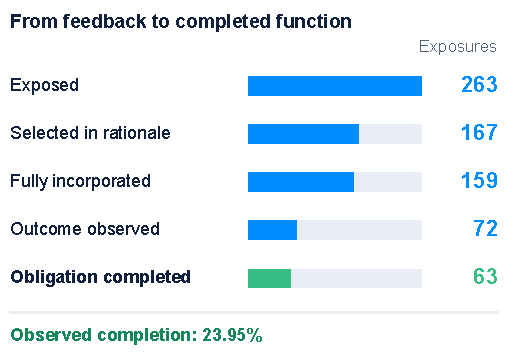
\includegraphics[width=\columnwidth]{fig2_requirements_flow.pdf}
\caption{Nested requirement exposure sets across 65 edits. Completion concerns the exposed obligation in observed successors. Another 20 complete incorporations lie outside the rationale-selected path. The 173 exposures without candidate execution are tracked separately from these stage counts.}
\label{fig:requirements}
\end{figure}

Each stage determines what the agent can carry forward. In the HR source, the omitted deferral must reach the editor as a failure before it can become a repair objective. An inherited guard needs usable task information and a matching runtime event to change an action. A later task introduces its own object and authority: a procedure learned for one announcement can prescribe the wrong action under a new instruction. The obligation gives us a common reference for tracing these changes from the original failure to the later action.

\section{System and evidence}
\label{sec:evidence}

\subsection{Two decisions through which evaluation controls learning}

\Gnosis{} stores textual units and executable components in versioned collections. A working collection retains edits, while a released collection advances through independent comparisons. Units specify runtime hooks and activation scope. Text can enter a model request; executable components can change arguments or observations and issue the task's original tool calls. The evaluator and permissions remain outside the agent's control.

The historical release rule requires observable improvement and zero task regression on six selection tasks, with two executions per task. A source must first succeed before a mature version comparison begins. In the frozen follow-up, strict failure on the source first run opens four editing slots, while strict success deploys the ancestor in all four. Every legal follow-up candidate is frozen before source retesting and transfer evaluation; source retests occur after deployment has been decided.

The eligible historical population contains 2,006 executions after the 7 October 2026 exclusion cutoff. The recovered graph has 130 vertices and 148 parent to child links across 211 version events. Proposal records include inspection actions as well as edits. Historical comparisons retain their batch conditions and task identities. The initial frozen evaluation, the subsequent interface studies, and the timing intervention are subsets of this historical population.

\subsection{Frozen intervention and business completion}

The follow-up uses one source from each of finance, HR, marketing, operations, sales, and support. Each source has four structurally related transfer tasks checked against all recorded prior exposure. All four editing conditions begin with the same ancestor, containing 13 textual units and one executable component. F0 supplies the complete source trajectory and assertion feedback. F1 retains those facts and adds a view organized by requirement, object, and action consequence. Its quotations resolve to the supplied source. R0 permits ordinary textual content. R1 requires nonempty \texttt{applies\_when}, \texttt{avoids}, and \texttt{guidance} fields in the JSON content of changed units; unchanged ancestor units persist verbatim. This treatment adapts the boundary representation of BASM~\cite{lin2026basm}.

The common limits are 24 units and 80,000 serialized characters; the ancestor occupies 65,524 characters. Format failure permits one retry and then retains the ancestor. All failures and untriggered slots remain in the workflow outcome. Seed 20261014 fixes the editing order and interleaves transfer evaluation within source blocks. Each of the four edit conditions, the ancestor, and the carry condition runs four tasks three times per block: 432 executions. Six source first runs and 24 retests give 462 in total. The protocol was sealed on 14 October 2026.

The follow-up model is \texttt{deepseek-flash}, accessed through DeepSeek's official API. Requests enable thinking with high reasoning effort and temperature 1. Each response permits up to 393,216 output tokens. AutomationBench~\cite{automationbench} is fixed at commit \texttt{4a8e106}, with its API toolset and at most 50 agent steps. Each run resets the task world and component state.

Task success requires all applicable obligations and normal termination, with execution errors counted as failures. Complete review defines obligations once per task and checks every run. A known failure fixes a failure label; remaining cases with unresolved obligations are unknown. Confirmed success uses all scheduled runs as its denominator. We retain original strict scoring and frozen assertion-indexed judgments alongside business review.

All 462 follow-up trajectories are replayed in the fixed official environment. Initial contracts, assertion outcomes, and strict success labels agree in $462/462$. The 63 historical executions with component effects also agree in $63/63$. Entity correspondence and runtime date differences remain separate from score agreement. An independent Codex agent checks 3,331 added obligation instances and reads 54 executions requiring semantic interpretation; 18 disagreements concern one quotation authority choice and alter one task label. The researcher reviews the final evidence. The supplement records provenance and all alternative authorization readings.

\section{Evaluation defines the reachable repairs}
\label{sec:selection}

\subsection{A missing obligation becomes a missing learning opportunity}

Let $h$ be a source trajectory, $Q(h)$ its binary evaluator score, and $B(h)$ its complete business outcome. In the follow-up, edit eligibility is $A(h)=1-Q(h)$. For current version $v$ and legal update operator $U$, the deployed version is
\begin{equation}
v'=
\begin{cases}
v, & Q(h)=1,\\
U(v,h), & Q(h)=0\text{ and generation succeeds},\\
v, & \text{generation fails}.
\end{cases}
\label{eq:eligibility}
\end{equation}
A false pass therefore changes the data generating process of learning. The omitted business failure receives no editing opportunity under this rule. Reformatting evidence downstream of $A$ leaves that decision intact.

In the HR source, the latest eligibility email requires an Airtable deferral for the employee on sabbatical and leaves courses unassigned. The first run creates four active employee records and omits that deferral. All nine assertions pass. Equation~\eqref{eq:eligibility} consequently closes all four editing slots, which deploy the ancestor. Every source retest repeats the business omission and passes the assertions. The unchanged content and the code path establish why this failure persists across the five observed executions.

The defect also gives the required correction a negative signal. Strict assertion 5 forbids \texttt{create\_record} for the employee targeted by the deferral. Creating the required record through that operation would fail the assertion. The source pass therefore suppresses an attempt, and the conflicting assertion penalizes the corrective action. Proposition~\ref{prop:exclusion} states the conditions under which this conflict restricts the functional variants available to the learner.

\begin{proposition}[Evaluator exclusion of a required correction]
\label{prop:exclusion}
Suppose business completion requires action $D$, evaluator success requires its absence, and a release rule preserves evaluator success on that task. From an evaluator-passing incumbent, every evaluated correction that performs $D$ on the protected task is excluded. Under Equation~\eqref{eq:eligibility}, an evaluator-passing source also produces zero edit attempts for that source, regardless of the available editing budget.
\end{proposition}

To see this, write $\mathcal B_D$ for trajectories satisfying the required action and $\mathcal Q$ for evaluator-passing trajectories. The hypotheses give $\mathcal B_D\subseteq\{D=1\}$ and $\mathcal Q\subseteq\{D=0\}$, hence $\mathcal B_D\cap\mathcal Q=\varnothing$. Preserving evaluator success excludes every corrective trajectory. The source statement follows directly from $A=0$. Removing the contradictory assertion removes this exclusion; changing the source eligibility rule removes the zero-attempt restriction. The HR execution instantiates the observed source restriction and the action conflict. Its four alternative edited lineages were never run.

\subsection{Feedback can teach the evaluator's error}

The sales source supplies the converse case. Under the main authorization reading, the latest Director instruction requires \texttt{MAJOR WIN}. The first run follows it and completes the business task. The original assertions demand \texttt{CLOSED} and prohibit \texttt{WIN:} and \texttt{MAJOR WIN:}, so editing begins. The editor's saved rationale explicitly cites the failed assertions, reclassifies the Director instruction as an unadopted suggestion, and elevates the older observed format to authority.

All three legal candidates rewrite that decision rule. F0R0 also installs a guard to normalize the announcement prefix. On source retest, all three strictly pass and violate the latest Director instruction. The fourth slot fails generation, retains the ancestor, and satisfies the business task while failing the assertions (Table~\ref{tab:source}). The edited candidates inherit the evaluator's interpretation through the editor's rationale and the resulting announcement rule.

\begin{table}[t]
\centering
\caption{Evaluation changes what is learned. Each entry is strict / complete business success. Sales uses the latest Director interpretation. Retests deploy the version recorded in the last column.}
\label{tab:source}
\footnotesize
\renewcommand{\arraystretch}{1.13}
\begin{tabular*}{\columnwidth}{@{\extracolsep{\fill}}llcc@{}}
\toprule
Source & Execution & Strict / business & Deployment\\
\midrule
HR & First run & $1/0$ & Ancestor\\
 & Four retests & $1/0$ in all four & Ancestor\\
\addlinespace
Sales & First run & $0/1$ & Ancestor\\
 & Three legal edits & $1/0$ in all three & Candidates\\
 & Failed generation & $0/1$ & Ancestor\\
\bottomrule
\end{tabular*}
\end{table}

The sales judgment follows the latest Director instruction. Under the older VP standard, \texttt{CLOSED} is correct. Sensitivity analysis evaluates all eight combinations of sales, quotation, and logging authority; the HR eligibility decision and the direction of the sales edits remain the same across these readings.

Across the 462 follow-up executions, complete review finds 262 confirmed successes, 179 failures, and 21 unknown outcomes. There are 102 strict passes with confirmed business failure and 38 strict rejections with confirmed business success. All 21 unknown runs strictly pass and remain outside those 102 errors. The source cases show how these disagreements affect learning: the score controls whether editing begins, and its assertions can become future guidance.

\subsection{A saturated evaluator stops acceptance before money runs out}

The earlier release experiment exposes a second restriction on reachable improvement. Both repair groups use a USD~8.5 allowance. The global validation group spends USD~3.028831 and GNOSIS USD~4.310552 before their released selection scores reach $12/12$. Their final comparisons give maximal candidate and reference scores and abstain. The remaining allowances are USD~5.471169 and USD~4.189448, respectively. GNOSIS's frozen held-out score is $101/150$: saturation of the 12 selection observations coexists with 49 failures in held-out execution.

Once every score used by a strict improvement rule reaches its maximum on a fixed panel, the rule has exhausted its admissible increases. Cheaper validation leaves this ceiling intact. Further accepted improvement requires feedback that can distinguish candidates at the remaining business failures.

\section{Usable experience depends on runtime and task authority}
\label{sec:expression}

After construction, a candidate must reach execution and satisfy an applicable obligation. The runtime studies follow its validation dependencies and component effects through to application state.

\subsection{Validation locality is a property of information flow}

Selective regression testing depends on the consumers of a change~\cite{ekstazi}. For changed agent units $\Delta$, let $\mathcal I(u)$ contain historical executions whose runtime inputs or actions can depend on unit $u$. The validation set is
\begin{equation}
\mathcal V(\Delta)=\bigcup_{u\in\Delta}\mathcal I(u).
\label{eq:union}
\end{equation}
Globally exposed changes make every task a consumer. Declaring narrow intent leaves this dependency intact whenever the runtime still exposes the changed content to the entire panel.

All 48 historical GNOSIS candidate validation plans rerun the complete panel and reuse zero executions. Three independently learned source repairs in the locality study all remain global and cover $36/36$ audit runs each. A subsequent scope interface comparison produces 19 legal candidates, every one containing global content; its eight mature candidates all require $12/12$ audit runs. Changing the declaration format leaves the runtime dependency broad.

The 240-execution timing intervention tests the proposed explanation that local guidance arrived too late. It fixes eight repairs and compares global early, local early, local delayed, contract early with body delayed, and removed guidance. Local early is noninferior to global early: $+2.08\pp$, with interval $[-4.17,8.33]\pp$ at the prespecified ten point margin. The planning versus execution-detail interaction for local early minus delayed is $-4.17\pp$, $p=1.0$, interval $[-25.00,12.50]\pp$. The prespecified analysis finds no reproducible timing pattern. Host dependency sets still cover every task in each of the eight audit pools, and routing plus prediction makes selective validation more expensive.

Early local access preserves utility under a fixed route. Every audit task still depends on the changed content, so routing saves zero validation runs. Selective validation requires some consumers to remain independent of the whole change. Equation~\eqref{eq:union} locates the observed burden in this information flow.

\subsection{Executable inheritance can preserve an inactive procedure}

Across history, 27 executable units enter 447 executions and produce 196 effects in 63 distinct executions; components themselves issue 27 tool calls. Of the 13 effect-bearing runs covered by complete business review, six succeed and seven fail. The runtime supports interventions, whose business consequences require a further check.

The inherited \texttt{ace\_op\_vp\_guard} receives 27,500 invocations across history and follow-up, with zero effects and zero component tool calls. The count separates into 720 task starts, 26,745 URLs outside its target branch, and 35 target URLs. Of the target cases, 23 obtain no usable prefix, ten already have the correct prefix, and two have invalid JSON bodies. The host passes \texttt{ctx.task} as an object, while the component reads \texttt{String(ctx.task)} and obtains \texttt{[object Object]}. The intended instruction is lost at the interface. Isolated replay of the original code in 45 saved real contexts reproduces zero argument changes and zero calls; all ten task starts reproduce that object conversion.

\subsection{Shared interfaces leave business decisions task dependent}

The subsequent frozen comparison on 18 new tasks makes the distinction between operational and business transfer visible. GNOSIS reduces failed tool calls from 651 to 112 and average actions from 75.14 to 39.31, while strict success stays at $20/36$ (Table~\ref{tab:efficiency}). Its execution expenditure falls from CNY~7.8513 to CNY~3.2733. Across 377 matched parent and candidate comparisons, 217 reduce tool failures; 159 of those do so without increasing strict success. These comparisons retain their shared execution identities.

\begin{table}[t]
\centering
\caption{Operational improvement and task completion on the same 18 tasks, two runs each. Failed calls are totals; actions are means; expenditure covers the 36 executions in CNY.}
\label{tab:efficiency}
\footnotesize
\renewcommand{\arraystretch}{1.13}
\begin{tabular*}{\columnwidth}{@{\extracolsep{\fill}}lrrrr@{}}
\toprule
Agent & Failed calls & Actions & Success & Cost\\
\midrule
Fixed & 651 & 75.14 & $20/36$ & 7.8513\\
Global & 165 & 45.47 & $25/36$ & 3.9763\\
GNOSIS & 112 & 39.31 & $20/36$ & 3.2733\\
\bottomrule
\end{tabular*}
\end{table}

Business completion requires the right operation on the right object under the current authority. Successful interface use addresses the first of these conditions. The inherited rule must still identify which document controls the task and which entities or exceptions it covers. The target task can reverse the source decision while using the same application (Table~\ref{tab:authority}). All 24 transfer tasks receive a reading against candidate contents and their own authorized materials.

\begin{table*}[t]
\centering
\caption{Authority and identity conditions change across tasks. Source rules occur in edited candidate content; target requirements come from the frozen task materials.}
\label{tab:authority}
\footnotesize
\renewcommand{\arraystretch}{1.18}
\begin{tabularx}{\textwidth}{@{}lLL@{}}
\toprule
Requirement & Inherited source decision & Authorized target decision\\
\midrule
Sales authority & Ignore account notes that redirect a deal announcement; retain the established announcement channel. & The DocuSign completion runbook explicitly authorizes account notes to determine credit holds and partner billing.\\
\addlinespace
Support identity & Group duplicates by exact email; records from different email addresses remain separate. & The cross-platform deduplication task supplies an alias table identifying different addresses as one customer and requires reciprocal internal notes.\\
\bottomrule
\end{tabularx}
\end{table*}

Several candidates retain source literals and authority decisions. Table~\ref{tab:authority} identifies target conditions under which those rules require revision. The aggregate experiment measures the full workflow across all tasks, including sources that retain the ancestor.

\section{Transfer tests the function constructed from source feedback}
\label{sec:transfer}

\subsection{The organization intervention changes a restricted part of learning}

Detailed assertion feedback enters edit rationales in $154/187$ exposures (82.35\%), compared with $7/70$ task summaries (10.00\%). Twelve of 17 repeatedly exposed requirement groups are never selected. This motivates the organization intervention: F0 and F1 receive the same complete facts, and F1 adds an organized view after eligibility. Both conditions retain the eligibility rule and the destination task's authority.

Twelve of the 24 slots never enter editing because HR, marketing, and operations strictly pass. The other 12 slots produce nine legal candidates and three terminal format failures, all under R1. Six R0 candidates change 51 units; three legal R1 candidates each change one. All slots retain their observed deployment in Table~\ref{tab:transfer}. The treatment includes its generation burden and the updates it actually produces.

For source block $b$, the primary difference averages four transfer tasks and three repetitions, then averages equally across the six blocks:
\begin{equation}
\begin{aligned}
d_b&=\frac{1}{12}\sum_{t=1}^4\sum_{r=1}^3
\bigl(y_{btr,\mathrm{F1R0}}-y_{btr,\mathrm{F0R0}}\bigr),\\
\widehat\Delta&=\frac{1}{6}\sum_b d_b.
\end{aligned}
\label{eq:effect}
\end{equation}
The frozen test enumerates 64 sign assignments, with a 95\% common shift inversion interval on a 0.0001 grid. Inference assumes exchangeable block signs and a common shift. The prespecified practical target is $+10\pp$.

\begin{table*}[t]
\centering
\caption{Full workflow outcomes on 24 transfer tasks, 72 runs per condition. Percentages use the complete denominator, including unknown outcomes. Every editing slot retains its actual deployment.}
\label{tab:transfer}
\footnotesize
\renewcommand{\arraystretch}{1.14}
\begin{tabular*}{\textwidth}{@{\extracolsep{\fill}}lrrrrrr@{}}
\toprule
& \multicolumn{2}{c}{Source deployment slots} & \multicolumn{2}{c}{Original and frozen evaluation} & \multicolumn{2}{c}{Complete business review}\\
\cmidrule(lr){2-3}\cmidrule(lr){4-5}\cmidrule(l){6-7}
Condition & Legal edits & Ancestor & Strict success & Frozen success & Confirmed success & Unknown\\
\midrule
F0R0 & 3 & 3 & 56 (77.8) & 58 (80.6) & 41 (56.9) & 4\\
F1R0 & 3 & 3 & 49 (68.1) & 51 (70.8) & 40 (55.6) & 4\\
F0R1 & 1 & 5 & 51 (70.8) & 53 (73.6) & 43 (59.7) & 3\\
F1R1 & 2 & 4 & 45 (62.5) & 47 (65.3) & 36 (50.0) & 2\\
\addlinespace
Ancestor / fresh retry & --- & 6 & 51 (70.8) & 55 (76.4) & 41 (56.9) & 4\\
Carry & --- & 6 & 72 (100.0) & 72 (100.0) & 49 (68.1) & 4\\
\bottomrule
\end{tabular*}
\end{table*}

Under frozen judgments, F1R0 minus F0R0 is $-9.72\pp$, $p=0.25$, interval $[-33.33,8.33]\pp$. Its upper endpoint is below the practical target, so organization fails the prespecified decision. Complete business review gives $-1.39\pp$, $p=1.0$, interval $[-25.00,8.33]\pp$. The alternative quotation authority gives zero difference and interval $[-25.00,16.66]\pp$. Assigning unknown obligations to minimize or maximize the contrast bounds the observed difference by $[-6.94,4.17]\pp$; the maximizing assignment has interval $[-8.33,16.66]\pp$.

The three sources that trigger editing average a $+2.78\pp$ business contrast; those retaining the ancestor average $-5.56\pp$ (Figure~\ref{fig:contrast}). The latter have identical content and inputs across conditions, so their differences arise in execution. Sixty groups with the same version, task, initial state, and input cover 360 paid runs; 328 of 1,548 within-group pairs change frozen labels (21.19\%). These pairs share executions. The R1 simple increment and interaction have Holm adjusted $p=1.0$, and no block supplies four legal edited candidates. The negative result concerns the full implemented workflow, including unchanged deployments and failed generation.

\begin{figure}[t]
\centering
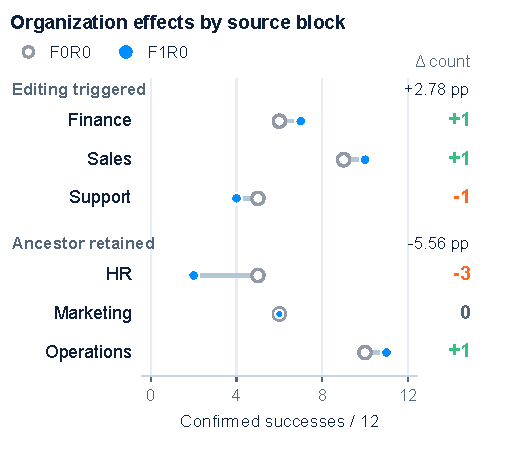
\includegraphics[width=\columnwidth]{fig3_contrast_blocks.pdf}
\caption{Business success under F0R0 and F1R0, grouped by actual editing eligibility. Each source block has 12 runs per condition. The right column gives count differences; group headings report mean differences in percentage points. Ancestor-retaining blocks use identical artifacts and inputs.}
\label{fig:contrast}
\end{figure}

\begin{figure*}[!t]
\centering
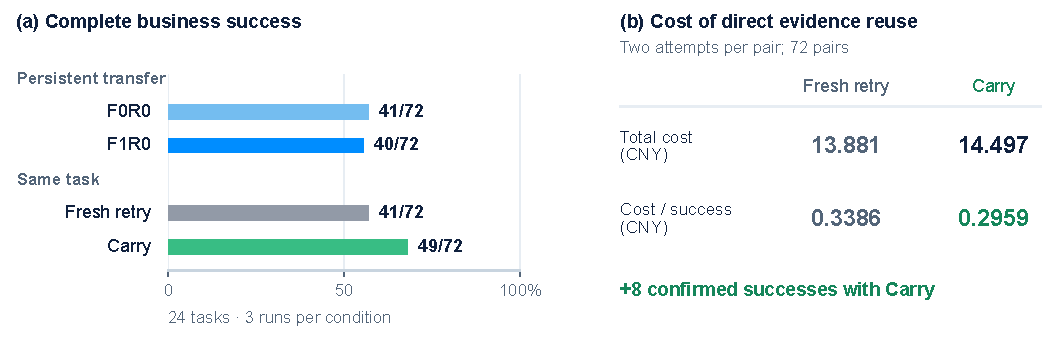
\includegraphics[width=\textwidth]{fig4_transfer_vs_carry.pdf}
\caption{Persistent transfer and direct task evidence. (a) Confirmed business success uses all 72 scheduled runs per condition. F1R0 adds organized source feedback; Carry receives the preceding trajectory and evaluator feedback for the same task. (b) Actual costs of 72 two-attempt pairs, including the first attempt. Carry buys eight additional confirmed successes for CNY~0.615916 more and lowers cost per confirmed success.}
\label{fig:transfer}
\end{figure*}

\subsection{Direct task evidence supports correction}

Carry receives its preceding ancestor trajectory with actions, tool returns, and assertion feedback, then restarts the original task world. Fresh retry uses the three ancestor runs in a fixed cyclic pairing per task. The 72 pairs therefore contain 72 distinct ancestor runs, each used once as a first attempt and once as another pair's retry. Aggregation preserves this sharing.

Carry raises frozen success from $55/72$ to $72/72$. Nine extra successes follow a failed first run and eight follow a passing first run. Complete business success increases from $41/72$ to $49/72$. The complete two-attempt cost increases from CNY~13.881212 to CNY~14.497128, or CNY~0.008554 per pair. Cost per confirmed success falls from CNY~0.338566 to CNY~0.295860. The prespecified lower total cost criterion fails; the observed benefit is eight additional confirmed successes for CNY~0.615916 more.

Direct evidence improves the fixed model's next attempt on the same task (Figure~\ref{fig:transfer}). Transfer additionally requires an inherited decision to remain valid when objects and authority change. F1 organizes the source facts; execution must still establish whether the resulting guidance applies at the destination.

\section{Acquisition and retention of business function}
\label{sec:functional}

Across all successors of the candidates traced in Section~\ref{sec:construction}, 117 requirement and execution observations contain 92 passes, 12 failures, 12 summaries without an identifiable requirement, and one unloaded component. Twenty requirement successes occur inside whole task failures. An agent can satisfy one obligation while failing another required for task success. Tracing individual requirements preserves these partial achievements for later comparison.

Retention begins at a verified functional success. Among 83 original assertion sequences, 54 have a subsequent applicable opportunity and 43 show no later failure, a conditional retention rate of 79.63\%. The other 29 lack follow-up. Expanded tracing of 196 event sequences gives 111 retained, 19 later failed, 60 without a successor, and six without a verified starting success. These observations establish that some completed functions persist across versions. Their opportunity counts distinguish sustained function from a version that simply continues to contain an artifact.

The protocol follows each obligation through the decisions needed to establish accumulated function. Task materials supply its authority; the score controls eligibility. The rationale and version difference show what the editor constructs. Successor inputs and component effects locate its expression, and application state establishes completion. Later applicable opportunities test retention; new tasks test the validity of transferred decisions. Failed generation and unchanged deployments retain their expenditure and outcomes.

\section{Related work}

Reflexion~\cite{reflexion}, ACE~\cite{ace}, and Voyager~\cite{voyager} establish verbal and executable carriers of experience. EASE~\cite{xiong2026ease} studies skill curation conditioned on downstream executor behavior. BASM~\cite{lin2026basm} represents applicability and failure conditions within retrieval and action checking. R1 changes how edited units are represented; its outcomes include failed generation and unchanged ancestor deployments.

Agent Plasticity~\cite{singh2026agentplasticity} studies inheritance and acquisition efficiency, including failures despite relevant artifacts. EvoPathBench~\cite{lin2026beyondendpoint} measures acquisition and retention alongside the gap between candidate improvements and selected updates. SkillScriptBench~\cite{liu2026skillscriptbench} follows documentation and script repair through preservation. We extend these process questions to business obligation identities and the control decisions that determine whether a repair is attempted.

Execution Consistency~\cite{yu2026executionconsistency} follows information through use and obligation completion. GAUGE~\cite{bodhwani2026gauge} studies evaluation validity and candidate rankings; VeriHarness~\cite{zhang2026veriharness} checks disputed claims and omissions against environmental evidence. SilentProbe~\cite{li2026silentprobe} studies failures despite apparently valid API behavior. We trace the evaluator's judgment into a persistent change, retaining obligations whose learning opportunity closes before an edit exists. Our validation argument draws on regression test selection~\cite{ekstazi}: the consumers of edited content determine the validation set.

\section{Conclusion}

Evaluation controls which business errors become learning objects and which interpretation enters persistent experience. In GNOSIS, the HR eligibility branch suppresses a needed correction. The sales edits inherit a scoring interpretation that reverses the latest Director instruction. A saturated selection panel also stops acceptance while money and held-out failures remain.

Following each obligation from feedback through runtime expression establishes where an inherited artifact supplies function. Later applicable opportunities test whether that function persists. Direct task evidence improves the next attempt, while the implemented organization treatment misses its transfer target.

\balance
\input{gnosis.bbl}
\clearpage
\nobalance
\appendix
\raggedbottom
\section{Evaluation protocol}\label{app:protocol}

The task partition uses seed 100 and the AutomationBench revision
\texttt{4a8e1061254004d9dac807054eed33fad7d1ff14}.
Table~\ref{tab:task-partition} gives every task identifier. Each domain contributes five development tasks, one independent selection task, and five final evaluation tasks. The six intermediate evaluation tasks are the first development task in each domain. Their evaluation outcomes are stored separately and are not supplied as repair feedback. Development evidence for those tasks remains available through the ordinary learning procedure.

\begin{table*}[t]
\centering
\caption{Fixed task partition. Identifiers are shown in full. A dagger marks the six development tasks used for intermediate evaluation. The development and final evaluation columns each contain 30 tasks; the independent selection set contains six tasks.}
\label{tab:task-partition}
\footnotesize
\setlength{\tabcolsep}{4pt}
\begin{tabularx}{\textwidth}{@{}XX@{}}
\toprule
Development & Final evaluation \\
\midrule
\path{sales.linkedin_profile_enrichment}$^{\dagger}$ & \path{sales.soft_matching} \\
\path{sales.chatgpt_contract_summary} & \path{sales.linkedin_event_promotion} \\
\path{sales.slack_deal_notification} & \path{sales.cross_reference_validation} \\
\path{sales.sheets_reconciliation} & \path{sales.docusign_void_resend} \\
\path{sales.mark_vip_emails_read} & \path{sales.send_customer_email} \\
\addlinespace
\path{operations.facebook_roas_monitoring}$^{\dagger}$ & \path{operations.space_utilization_analysis} \\
\path{operations.purchase_order_three_way_match} & \path{operations.office_supply_budget_monitoring} \\
\path{operations.twilio_afterhours_incident} & \path{operations.fire_extinguisher_inspection_schedule} \\
\path{operations.drive_slack_dock_schedule} & \path{operations.hubspot_personalized_outreach} \\
\path{operations.calendar_slack_training} & \path{operations.sheets_asana_approved_request} \\
\addlinespace
\path{hr.airtable_learning_path_assignment}$^{\dagger}$ & \path{hr.slack_channel_onboarding} \\
\path{hr.promotion_announcement} & \path{hr.performance_feedback_logging} \\
\path{hr.airtable_skills_matrix} & \path{hr.employee_request_routing} \\
\path{hr.policy_update_distribution} & \path{hr.interview_scheduling} \\
\path{hr.mandatory_meeting_compliance} & \path{hr.salary_adjustment_processing} \\
\addlinespace
\path{marketing.customer_milestone}$^{\dagger}$ & \path{marketing.social_engagement_response} \\
\path{marketing.landing_page_conversion} & \path{marketing.partner_comarketing} \\
\path{marketing.competitive_response_plan} & \path{marketing.event_followup_personalization} \\
\path{marketing.seasonal_campaign} & \path{marketing.influencer_contract_tracking} \\
\path{marketing.content_syndication} & \path{marketing.social_content_calendar} \\
\addlinespace
\path{support.gorgias_channel_consolidation}$^{\dagger}$ & \path{support.zendesk_maintenance_notify} \\
\path{support.hiver_coaching_pipeline} & \path{support.reamaze_intercom_migration} \\
\path{support.freshdesk_sla_monitoring} & \path{support.helpscout_jira_bugs} \\
\path{support.intercom_freshdesk_escalation} & \path{support.hiver_response_sla} \\
\path{support.gorgias_freshdesk_migration} & \path{support.zendesk_hubspot_churn_risk} \\
\addlinespace
\path{finance.prepaid_amortization}$^{\dagger}$ & \path{finance.wave_client_statement} \\
\path{finance.project_profitability} & \path{finance.qb_undeposited_funds} \\
\path{finance.invoice_file_organization} & \path{finance.gl_variance_analysis} \\
\path{finance.qb_invoice_from_orders} & \path{finance.monday_project_billing} \\
\path{finance.xero_credit_allocation} & \path{finance.vendor_payment_approval} \\
\midrule
\multicolumn{2}{@{}l}{Independent selection} \\
\path{sales.chatgpt_lead_summary_generator} & \path{operations.cross_department_budget_reconciliation} \\
\path{hr.compliance_training_enforcement} & \path{marketing.content_localization} \\
\path{support.helpcrunch_engagement_scoring} & \path{finance.dept_expense_rollup} \\
\bottomrule
\end{tabularx}
\end{table*}

All four frozen conditions use the official DeepSeek API with model identifier \texttt{deepseek-flash}, reasoning enabled at \texttt{high} effort, temperature 1, and a maximum output of 393,216 tokens per response. This output limit is distinct from the model's context capacity. The benchmark uses the \texttt{api} toolset and allows at most 50 agent steps. Each evaluation starts with a fresh environment and fresh component state. Previous evaluation responses and trajectories are absent from subsequent independent executions. These conditions define the comparison: changing the initial state or exposing prior evaluation outcomes changes the task-solving distribution being measured.

The frozen conditions each run the same 30 tasks five times, yielding 150 executions per condition and 600 executions in total. All 600 terminate normally. The development execution check completes 30 tasks, with 21 strict successes and no truncation among the nine failures. Final evaluation uses the frozen versions in Table~\ref{tab:frozen-versions}; intermediate evaluation uses a separate working candidate, \texttt{986335b24f89}. Fingerprints are abbreviated to 12 hexadecimal characters, which distinguish all versions listed here. The experiment implementation fingerprint begins \texttt{0d4c2efbc3b1}, and its Git history includes commit \texttt{4f742b9}.

\begin{table}[t]
\centering
\caption{Frozen versions used in all five independent repetitions. Text and executable counts describe persistent units.}
\label{tab:frozen-versions}
\footnotesize
\begin{tabular}{@{}llrr@{}}
\toprule
Condition & Fingerprint & Text & Executable \\
\midrule
Fixed & \texttt{4f53cda18c2b} & 0 & 0 \\
ACE & \texttt{9b29cc26db48} & 1 & 0 \\
Global & \texttt{341e767a59ec} & 17 & 0 \\
GNOSIS & \texttt{0faf0fdd660e} & 13 & 1 \\
\bottomrule
\end{tabular}
\end{table}

The repeated-attempt condition retains the preceding trajectory for revision and scores the last attempt on each task. It makes 354 attempts: 347 end normally, six reach the allocated task budget, and one is truncated. The 30 final outcomes comprise 23 normal terminations, six budget terminations, and one truncation. Its success rate therefore uses 30 final outcomes, while the frozen conditions use 150 independent outcomes summarized within 30 tasks.

\section{Statistical results}\label{app:statistics}

For task $i$ and condition $g$, strict performance is the mean of the five binary outcomes, $s_{ig}=\frac{1}{5}\sum_{r=1}^{5}y_{igr}$. Partial credit is averaged over the same five repetitions. Comparisons use the 30 task differences $d_i=s_{i,\mathrm{GNOSIS}}-s_{ig}$. The two-sided exact paired permutation test enumerates every sign assignment to nonzero task differences. Paired bootstrap intervals resample the 30 task pairs 200,000 times with NumPy seed 100. This preserves the repeated observations belonging to each task.

Table~\ref{tab:complete-statistics} reports all three comparisons for each endpoint. Holm adjustment is performed separately within each endpoint's family of three comparisons. The all-five-success endpoint is binary at the task level and uses the two-sided exact McNemar test. Its discordant counts indicate tasks for which GNOSIS alone or the comparison condition alone succeeds in every repetition. GNOSIS has the highest observed strict success and the most consistently solved tasks; none of the Holm-adjusted comparisons reaches 0.05.

\begin{table*}[t]
\centering
\caption{Complete task-level comparisons of GNOSIS against each frozen condition. Strict differences and their intervals are in percentage points. Partial-credit differences use the original $[0,1]$ scale. For all-five success, the effect column gives discordant wins/losses.}
\label{tab:complete-statistics}
\small
\begin{tabular}{@{}llrlrr@{}}
\toprule
Endpoint & Comparator & \shortstack{Difference or\\wins/losses} & \shortstack{95\% paired\\bootstrap interval} & Exact $p$ & Holm $p$ \\
\midrule
Strict success & Fixed & $+3.3333$ & $[-4.0000,10.0000]$ & 0.472656 & 0.656250 \\
 & ACE & $+8.0000$ & $[-2.6667,19.3333]$ & 0.218750 & 0.656250 \\
 & Global & $+5.3333$ & $[-2.0000,12.6667]$ & 0.242188 & 0.656250 \\
\addlinespace
Partial credit & Fixed & $+0.047386$ & $[0.012508,0.085662]$ & 0.016914 & 0.050743 \\
 & ACE & $+0.055867$ & $[0.001575,0.108880]$ & 0.052208 & 0.104416 \\
 & Global & $-0.000534$ & $[-0.034793,0.028595]$ & 0.976685 & 0.976685 \\
\addlinespace
All-five success & Fixed & $8/1$ & --- & 0.039063 & 0.117188 \\
 & ACE & $7/1$ & --- & 0.070313 & 0.125000 \\
 & Global & $5/0$ & --- & 0.062500 & 0.125000 \\
\bottomrule
\end{tabular}
\end{table*}

\section{Components and selection}\label{app:components}

Every delivered unit has \texttt{GLOBAL} scope. The final GNOSIS version contains 13 text units and one executable E component, \texttt{ace\_op\_vp\_guard}, which processes job-title information at the task API boundary. Across development, the candidate history contains ten distinct executable source contents, including revisions of the same component. The host compiles the TypeScript source and registers it through Cordis; execution occurs in QuickJS with access to the task's original capabilities. During the 150 final GNOSIS executions, the executable component is invoked 6,276 times: 150 at task start and 6,126 before a tool call. These invocations produce zero nonempty effects and zero capability calls. The 13 text units are injected 1,950 times. Thus the executable component contributes no observed runtime intervention to the final evaluation.

Both repair conditions conduct four mature comparisons, each planning 12 candidate executions on the six selection tasks. All 48 GNOSIS plans start at the task beginning because the changed version includes globally active units. No historical execution is reused. The same counts hold for the global validation condition. Table~\ref{tab:selection-evolution} gives the release progression and the actual settled resource use. Selection means describe the accepted release sequence; the final comparison in each condition has candidate and incumbent means both equal to 1.0, producing abstention under the strict-improvement rule.

In chronological order, the four GNOSIS comparisons have incumbent/candidate success counts of $10/9$, $10/11$, $11/12$, and $12/12$, each out of 12 executions per side. The middle two candidates are accepted. Global has counts of $10/9$, $10/10$, $10/12$, and $12/12$; only the third candidate is accepted. Equal aggregate counts in Global's second comparison conceal a task-level regression, which prevents release under the zero-regression condition. Both conditions therefore finish at the maximum observed selection score.

\begin{table}[t]
\centering
\caption{Selection outcomes under the shared USD 8.5 learning allowance. Expenditure includes learning and selection.}
\label{tab:selection-evolution}
\footnotesize
\begin{tabularx}{\columnwidth}{@{}lXX@{}}
\toprule
Quantity & Global & GNOSIS \\
\midrule
Settled expenditure (USD) & 3.028831 & 4.310552 \\
Accepted releases & 1 & 2 \\
Mature comparisons & 4 & 4 \\
New candidate executions & 48 & 48 \\
Reused executions & 0 & 0 \\
Accepted selection means & $0.8333\to1.0$ & $0.8333\to0.9167\to1.0$ \\
Releases per USD & 0.330160 & 0.463978 \\
Unspent allowance (USD) & 5.471169 & 4.189448 \\
\bottomrule
\end{tabularx}
\end{table}

The intermediate evaluation compares an early version with the working candidate on the six marked development tasks. Strict success increases from four to five tasks, and mean partial credit increases from 0.934524 to 0.958333. The learning-path assignment and prepaid-amortization tasks change from failure to success. The customer-milestone task changes from success to failure, with partial credit 0.75. The remaining three tasks remain successful. These transitions characterize the intermediate working candidate, whose fingerprint differs from the final released version.

\section{Cost accounting}\label{app:cost}

Resource comparisons use settled token charges at fixed reference rates: CNY 1 per million uncached input tokens, CNY 0.02 per million cached input tokens, and CNY 4 per million output tokens. USD learning allowances are converted at CNY 7.1 per USD. Table~\ref{tab:stage-costs} separates experience formation from final execution. Selection charges are included in the learning-and-selection column and are also shown separately to expose that component of the total. Intermediate evaluation and fixed-candidate retesting are distinct stages.

\begin{table*}[t]
\centering
\caption{Settled reference expenditure by condition and stage, in CNY. The selection column is a subset of learning and selection and is not added again in the total.}
\label{tab:stage-costs}
\small
\begin{tabular}{@{}lrrrrrr@{}}
\toprule
Condition & \shortstack{Learning and\\selection} & \shortstack{Selection\\subset} & Intermediate & \shortstack{Final\\execution} & \shortstack{Fixed-candidate\\retest} & All stages \\
\midrule
Fixed & 6.059709 & 0 & 0 & 28.279199 & 0 & 34.338908 \\
ACE & 10.170880 & 0 & 0 & 24.111810 & 0 & 34.282690 \\
Global & 21.504698 & 7.001778 & 0 & 17.350725 & 2.400554 & 41.255977 \\
GNOSIS & 30.604922 & 5.410830 & 1.472953 & 14.194113 & 1.856502 & 48.128490 \\
Repeat & 0 & 0 & 0 & 45.831735 & 0 & 45.831735 \\
\bottomrule
\end{tabular}
\end{table*}

GNOSIS development plus final evaluation costs CNY 46.271988, including intermediate evaluation and excluding the separate fixed-candidate retest. Dividing by 30 assigns CNY 1.542400 to each repeated-attempt task. The repeated-attempt condition spends CNY 45.831735 in total, or CNY 1.527725 per task, leaving 0.951445\% of its allocation unused. The measured amortization curve has no crossing over the 1--30 task range. Mean frozen execution charges are CNY 0.188528 for Fixed, 0.160745 for ACE, 0.115672 for Global, and 0.094627 for GNOSIS.

Official account exports give the cash expenditure in Table~\ref{tab:official-costs}. Dates use UTC+08:00; the October 8 amount is the snapshot available at export. The sum is CNY 206.71348282 across 18,467 requests. Cached input accounts for 91.43\% of the 828,635,115 input tokens. Input cache misses cost CNY 71.026074, cache hits cost CNY 15.15218082, and output costs CNY 120.535228.

\begin{table*}[t]
\centering
\caption{Official account usage and actual charges by date (UTC+08:00). Token counts and costs retain the precision of the exported totals.}
\label{tab:official-costs}
\small
\begin{tabular}{@{}lrrrrr@{}}
\toprule
Date & Requests & Uncached input tokens & Cached input tokens & Output tokens & Charge (CNY) \\
\midrule
2026-10-07 & 4,182 & 31,201,724 & 192,144,768 & 8,017,475 & 67.11451936 \\
2026-10-08 & 14,285 & 39,824,350 & 565,464,273 & 22,116,332 & 139.59896346 \\
\midrule
Total & 18,467 & 71,026,074 & 757,609,041 & 30,133,807 & 206.71348282 \\
\bottomrule
\end{tabular}
\end{table*}

The local ledger contains 18,133 call records, of which 18,127 have settled charges totaling CNY 203.837800. Six unsettled reservations sum to CNY 9.727237: CNY 3.286512 for ACE and CNY 6.440725 for Global. Reservations are excluded from every settled total in Table~\ref{tab:stage-costs}. The official exports exceed the local settled reference total by CNY 2.875683 and contain 334 more requests. They provide daily aggregates without request identifiers or experimental-condition fields, so this difference remains at the account level. Condition-level comparisons use the local phase assignments. The local time-of-day estimate of CNY 226.488652 is separate from the official cash total; the daily exported usage reproduces the official charges directly at the stated token prices.

\end{document}
